\chapter{Perception of word-final /s/}\label{chapter06}

As introduced in detail in Section \ref{section02_2}, the perception study presented here investigates whether subphonemic durational differences in word-final /s/ are perceived by listeners. Two hypotheses derived from theories and models of speech perception are examined. \textsc{H perc\textsubscript{1}}, the ``Abstractionist Hypothesis", assumes that listeners are not sensitive to subphonemic durational differences. \textsc{H perc\textsubscript{2}}, the ``Phonetic Detail Hypothesis", predicts that subphonemic durational differences are perceptible. Subsequently, listeners are assumed to be sensitive to such differences. The two hypotheses are tested by analysing the results of a same-different task.

\section{Methodology}\label{section06_1}

\subsection{Participants}\label{section06_1_1}

Forty native speakers of New Zealand English took part in the same-different task. One participant had to be excluded right away as they did not respond in any trial. The mean age of the remaining 39 subjects was 23.0 years, ranging from 18 to 39. Six participants identified as multilingual. The experiment took place at the University of Canterbury, Christchurch, New Zealand, from December 2020 to March 2021. 

\subsection{Materials}\label{section06_1_2}

The speech materials consisted of pseudowords as well as of real words and real word filler items. As the aim of the present experiment was to study the perception of word-final /s/, only those pseudowords with word-final /s/ were used. The 24 pseudowords used as stimuli were introduced in Section \ref{section03_1_2}. For reasons of convenience, Table \ref{tab:6.1} lists these pseudowords once more.

\begin{table}\fontsize{10}{11}
\caption{Orthographic (\textit{orth.}) and phonological (\textit{phon.}) representations of the pseudowords used in the same-different task.}
\label{tab:6.1}
\centering
\begin{tabular}{lllllll} 
\lsptoprule
~              & /glɪ/          & /prʌ/          & /pli:/          & /clu:/          & /blaʊ/          & /gleɪ/           \\ 
\midrule
\textit{orth.} & \textit{glips} & \textit{prups} & \textit{pleeps} & \textit{cloops} & \textit{bloups} & \textit{glaips}  \\
\textit{phon.} & /glɪps/        & /prʌps/        & /pli:ps/        & /klu:ps/        & /blaʊps/        & /gleɪps/         \\ 
\midrule
\textit{orth.} & \textit{glits} & \textit{pruts} & \textit{pleets} & \textit{cloots} & \textit{blouts} & \textit{glaits}  \\
\textit{phon.} & /glɪts/        & /prʌts/        & /pli:ts/        & /klu:ts/        & /blaʊts/        & /gleɪts/         \\ 
\midrule
\textit{orth.} & \textit{gliks} & \textit{pruks} & \textit{pleeks} & \textit{clooks} & \textit{blouks} & \textit{glaiks}  \\
\textit{phon.} & /glɪks/        & /prʌks/        & /pli:ks/        & /klu:ks/        & /blaʊks/        & /gleɪks/         \\ 
\midrule
\textit{orth.} & \textit{glifs} & \textit{prufs} & \textit{pleefs} & \textit{cloofs} & \textit{bloufs} & \textit{glaifs}  \\
\textit{phon.} & /glɪfs/        & /prʌfs/        & /pli:fs/        & /klu:fs/        & /blaʊfs/        & /gleɪfs/         \\
\lspbottomrule
\end{tabular}
\end{table}

The set of twelve real words used in this experiment was also introduced in Section \ref{section03_1_2}. Recall that words were taken from the British National Corpus (\cite{Davies2004}), following a number of criteria. That is, words had to have a word-final /s/ as part of a voiceless stop plus sibilant coda; they had to be either singular or plural nouns with one syllable; and the number of short monophthong, long monophthong, and diphthong nuclei had to be equally distributed across words for both singular and plural nouns. For singular /s/, it was not possible to fully meet the final criterion as there was only one word with a long monophthong nucleus. Another monomorphemic word with a short monophthong was used instead. The set of real words is given in Table \ref{tab:6.2}.

\begin{table}\fontsize{10}{11}
\caption{Real words used in the same-different task.}
\label{tab:6.2}
\centering
\begin{tabular}{llll} 
\lsptoprule
\multicolumn{2}{c}{Non-morphemic /s/} & \multicolumn{2}{c}{Plural suffix /s/}  \\ 
\midrule
Item            & Vowel quality       & Item            & Vowel quality        \\
\midrule
\textit{mix}    & short               & \textit{books}  & short                \\
\textit{box}    & short               & \textit{steps}  & short                \\
\textit{tax}    & short               & \textit{rights} & diphthong            \\
\textit{coax}   & diphthong           & \textit{points} & diphthong            \\
\textit{hoax}   & diphthong           & \textit{groups} & long                 \\
\textit{corpse} & long                & \textit{parts}  & long                 \\
\lspbottomrule
\end{tabular}
\end{table}

Additionally, twelve filler items were employed. All filler items were singular nouns consisting of a single syllable with either a short monophthong, a long monophthong, or a diphthong as nucleus. The nucleus type followed the same distribution as for the items described above, i.e. one third of filler items per type of nucleus. Half of the filler items ended in /f/, while the other half ended in /θ/. See Table \ref{tab:6.3} for all filler items.

\begin{table}\fontsize{10}{11}
\caption{Filler items used in the same-different task.}
\label{tab:6.3}
\centering
\begin{tabular}{llll} 
\lsptoprule
\multicolumn{2}{c}{Non-morphemic /s/} & \multicolumn{2}{c}{Plural suffix /s/}  \\ 
\midrule
Item            & Vowel quality       & Item            & Vowel quality        \\
\midrule
\textit{riff}    & short               & \textit{death}  & short                \\
\textit{muff}    & short               & \textit{myth}  & short                \\
\textit{wife}    & diphthong               & \textit{faith} & diphthong            \\
\textit{safe}   & diphthong           & \textit{growth} & diphthong            \\
\textit{grief}   & diphthong           & \textit{booth} & long                 \\
\textit{hoof} & long                & \textit{path}  & long                 \\
\lspbottomrule
\end{tabular}
\end{table}

The recording of the speech materials took place at a soundproof booth of the Department of Linguistics at the University of Tübingen. For this, reading lists were created. On these lists, items were embedded within the sentence ``He said \textit{item} to me.". A trained native speaker of New Zealand English read the entire reading list aloud for practice before recording the list three times. The recordings were sampled at 44.1 kHz, 16 bit.

For each item the best of the three recordings was chosen by manual inspection. First, all recordings were analysed using Praat following the segmentation conventions laid out in Section \ref{section04_1_4}. Recordings with production errors, e.g. laughter, stutter or vocal fry, or segmentation difficulties were dismissed. Second, the remaining segmented target and filler items were spliced from their surrounding contexts, resulting in audio files only containing the words of interest. Third, the duration of the items and filler items was measured using a Praat script (\cite{deJong2008}) and then analysed in R. The result of this analysis is given as the mean durations presented in Table \ref{tab:6.4}. Lastly, for each item the version closest to the mean duration of its nucleus type was chosen for further use in the experiment to keep durational differences between items to a minimum.

\begin{table}\fontsize{10}{11}
\caption{Mean durations of items and filler items across recordings in seconds.}
\label{tab:6.4}
\centering
\begin{tabular}{llccc} 
\lsptoprule
Item type   & ~                                                                   & Short vowel                                           & Long vowel                                            & Diphthong                                              \\ 
\midrule
real words  & \begin{tabular}[c]{@{}l@{}}\textit{mean} \\\textit{sd}\end{tabular} & \begin{tabular}[c]{@{}l@{}}0.576 \\0.109\end{tabular} & \begin{tabular}[c]{@{}l@{}}0.613 \\0.102\end{tabular} & \begin{tabular}[c]{@{}l@{}}0.572 \\0.062\end{tabular}  \\ 
\midrule
pseudowords & \begin{tabular}[c]{@{}l@{}}\textit{mean} \\\textit{sd}\end{tabular} & \begin{tabular}[c]{@{}l@{}}0.521 \\0.060\end{tabular} & \begin{tabular}[c]{@{}l@{}}0.551 \\0.042\end{tabular} & \begin{tabular}[c]{@{}l@{}}0.550 \\0.046\end{tabular}  \\ 
\midrule
filler      & \begin{tabular}[c]{@{}l@{}}\textit{mean} \\\textit{sd}\end{tabular} & \begin{tabular}[c]{@{}l@{}}0.455 \\0.052\end{tabular} & \begin{tabular}[c]{@{}l@{}}0.490 \\0.067\end{tabular} & \begin{tabular}[c]{@{}l@{}}0.549 \\0.071\end{tabular}  \\
\lspbottomrule
\end{tabular}
\end{table}

In a next step, the final /s/ duration of all items was manipulated in such a way that it corresponded to the mean /s/ duration for non-morphemic and plural /s/ found in the reference study by \citet{Plag2017}. For example, in the case of \textit{mix} the duration of the final /s/ was changed to 318 ms, while in the case of \textit{books} the duration of the final /s/ was changed to 283 ms. This was done for all items, i.e. real words and pseudowords. 

Pseudowords were treated as both singular and plural nouns. That is, pseudowords were equally distributed across four groups as follows. First, each group consisted of at least one pseudoword ending in /ps/, /ts/, /ks/, and /fs/. Second, groups A and B had two additional pseudowords ending in /ps/ and /ts/, respectively, while groups C and D had two additional pseudowords ending in /ks/ and /fs/, respectively. See Table \ref{tab:6.5} for the distribution of pseudowords across groups. 

\begin{table}\fontsize{10}{11}
\caption{Pseudoword distribution across the groups A-D used in the same-different task.}
\label{tab:6.5}
\centering
\begin{tabular}{lcccc} 
\lsptoprule
~     & Group A & Group B & Group C & Group D  \\ 
\midrule
gli-  & ps      & ts      & ks      & fs       \\
plee- & ts      & ps      & fs      & ks       \\
cloo- & ks      & ts      & ps      & fs       \\
pru-  & fs      & ks      & ts      & ps       \\
blou- & ps      & fs      & ks      & ts       \\
glai- & ts      & ps      & fs      & ks       \\
\lspbottomrule
\end{tabular}
\end{table}

The pseudowords in groups A and C were treated as singular nouns with a non-morphemic word-final /s/, while the pseudowords in groups B and D were treated as plural nouns with a plural word-final /s/. Their /s/ durations were changed accordingly. This way of handling type of /s/ across pseudowords was chosen to keep priming effects across pseudowords to a minimum, i.e. no participant was to encounter pseudowords with both singular and plural /s/ durations. 

Then, four altered versions of each modified item were created. Each non-morphemic /s/ item was edited in such a way that 10 ms, 20 ms, 35 ms, or 75 ms were subtracted from the word-final /s/ duration, making it gradually more similar to plural word-final /s/ in terms of its duration. For plural /s/ items, 10 ms, 20 ms, 35 ms, or 75 ms were added to the word-final /s/ duration, making it gradually more similar to non-morphemic word-final /s/ in terms of its duration. This resulted in five different /s/ durations per recorded item. See Table \ref{tab:6.6} for all final /s/ durations across non-morphemic and plural /s/ items. Depending on the pertinent item, the duration of the word-final /s/ took up more than half of the total word duration (cf. Table \ref{tab:6.4} and Table \ref{tab:6.6}) and was notably longer than the original non-edited /s/ which showed a mean duration of 174 ms. Nonetheless, all items sounded natural. In total, five versions for each of the 12 real word items and for each of the 24 pseudoword items were created, resulting in 180 items. Each participant was to listen to 90 of them, i.e. (12 real words + 6 pseudowords) × 5 versions.

\begin{table}\fontsize{10}{11}
\caption{Durations in milliseconds for non-morphemic and plural /s/ for real word and pseudoword items.}
\label{tab:6.6}
\centering
\begin{tabular}{lccccc} 
\lsptoprule
~             & Mean & ± 10 ms & ± 20 ms & ± 35 ms & ± 75 ms  \\ 
\midrule
non-morphemic & 318  & 308     & 298     & 283     & 243      \\
plural        & 283  & 293     & 303     & 318     & 358      \\
\lspbottomrule
\end{tabular}
\end{table}

A similar approach was used for the manipulation of filler items. Their final fricative duration was altered as well. For this, the mean duration of word-final /f/ and /θ/ was measured after extracting the recorded filler items from their contexts. It was found that the mean duration of word-final /f/ was 244 ms, while the mean duration of /θ/ was 217 ms. It was therefore decided that the duration of /f/ was treated similarly to that of non-morphemic /s/, i.e. it was shortened, while the duration of /θ/ was treated similarly to that of plural /s/, i.e. it was lengthened. The different durations for both /f/ and /θ/ are given in Table \ref{tab:6.7}.

\begin{table}\fontsize{10}{11}
\caption{Durations in milliseconds for /f/ and /θ/ for filler items.}
\label{tab:6.7}
\centering
\begin{tabular}{lccccc} 
\lsptoprule
~             & Mean & ± 10 ms & ± 20 ms & ± 35 ms & ± 75 ms  \\ 
\midrule
/f/ filler items & 244  & 234     & 224     & 209     & 169      \\
/θ/ filler items & 217  & 227     & 237     & 252     & 292      \\
\lspbottomrule
\end{tabular}
\end{table}

\subsection{Procedure}\label{section06_1_3}

The same-different task was conducted in OpenSesame (\cite{Mathot2012}). First, participants were introduced to the same-different task. They were told that during the following experiment, they were to hear two recordings of the same word at a time and that they had to decide whether these two recordings were identical or different. It was explained that they should decide as quickly as possible and answer by pressing either the ``same" or ``different" key on the keyboard. The key assigned to ``same" was ``A", the key assigned to ``different" was ``K". The ``A" key was pressed using the left index finger, the ``K" key was pressed using the right index finger. Both options were given on screen during the entire experiment as illustrated by Figure \ref{fig:6_1}. The participants were also told that if they did not decide on either option within a certain amount of time, the next trial would start automatically. Each participant started with ten practice trials, which consisted of six pseudoword items for familiarisation and four filler items.

\begin{figure}
    \centering
    \includegraphics[width=0.7\textwidth]{figures/fig6.1.png}
    \caption{Option display during the perception experiment.}
    \label{fig:6_1}
\end{figure}

Each trial was preceded by a fixation cross and a stretch of silence of 450 ms. Then, both recordings played, with reaction time measurement starting at the onset of the second recording. The word-final /s/ of both recordings was either similar or different in duration, following one of the possible combinations given in Table \ref{tab:6.8}, resulting in a trial number of 270, i.e. (12 real word items + 6 pseudoword items + 12 filler items) × 9 combinations. The experiment was split into four main parts to allow for short pauses. Each part consisted of either 67 or 68 trials 
(67 × 2 + 68 × 2 = 270). Within each of the four parts, target and filler items were distributed evenly but pseudorandomised, i.e. it was prevented that two trials in a row neither contained the same target or filler item nor the same combination of /s/ durations.

\begin{table}\fontsize{10}{11}
\caption{Combinations of /s/ durations used in the same-different task. ``mean" is the mean duration found in \citet{Plag2017} for non-morphemic and plural /s/. ± represents a subtraction for non-morphemic /s/ items and an addition for plural /s/ items.}
\label{tab:6.8}
\centering
\begin{tabular}{llll}
\lsptoprule
Same/different & /s/ durations of items                                                     & Same/different & /s/ durations of items                                             \\
\midrule
same           & mean vs. mean                                                            & different      & \begin{tabular}[c]{@{}l@{}}mean vs.\\ mean ± 10 ms\end{tabular}  \\
same           & \begin{tabular}[c]{@{}l@{}}mean ± 10 ms vs. \\ mean ± 10 ms\end{tabular} & different      & \begin{tabular}[c]{@{}l@{}}mean vs.\\ mean ± 20 ms\end{tabular}  \\
same           & \begin{tabular}[c]{@{}l@{}}mean ± 20 ms vs. \\ mean ± 20 ms\end{tabular} & different      & \begin{tabular}[c]{@{}l@{}}mean vs.\\ mean ± 35 ms\end{tabular}  \\
same           & \begin{tabular}[c]{@{}l@{}}mean ± 35 ms vs. \\ mean ± 35 ms\end{tabular} & different      & \begin{tabular}[c]{@{}l@{}}mean vs.\\ mean ± 75 ms\end{tabular}  \\
same           & \begin{tabular}[c]{@{}l@{}}mean ± 75 ms vs. \\ mean ± 75 ms\end{tabular} & ~              & ~          \\
\lspbottomrule
\end{tabular}
\end{table}

Participants were given a 2,000 ms window to react, starting after the offset of the second recording. After that a time-out was recorded. The next trial automatically started 2,500 ms after the offset of the second recording if no reaction was recorded.

\section{Analysis}\label{section06_2}

Data of same-different tasks are often analysed in terms of their error-rates (e.g. \cite{Belke2002, Norris2008errorrates, Lupker2018}). For example, if a certain condition A shows a significantly higher error rate as compared to another condition B, it is concluded that perception of condition A is significantly worse. Figure \ref{fig:6_2} shows the overall error rates of the present same-different task results.

\begin{figure}
    \centering
    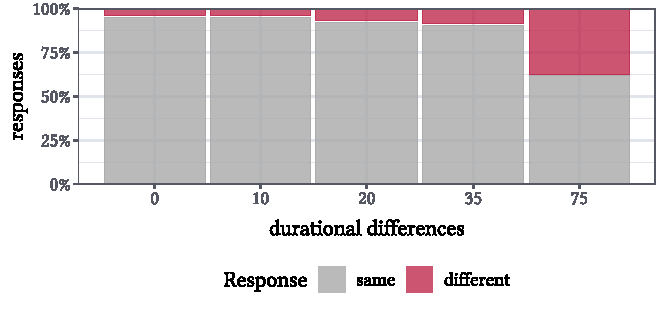
\includegraphics[]{figures/fig6.2.pdf}
    \caption{Overall error rates for the same-different task for all durational differences and across all subjects. For a durational difference of 0 ms the error rate is represented by the part of the bar corresponding to \texttt{different}, while for all other durational differences the error rate is the given part of the pertinent bars corresponding to \texttt{same}.}
    \label{fig:6_2}
\end{figure}

For a durational difference of 0 ms, the error rate is rather low with about 4\%. For the 10 ms difference, the error rate is 96\%; for the 20 ms difference, the error rate is 93\%; for the 35 ms difference, the error rate is 91\%; and for the 75 ms difference, the error rate is 62\%. However, the overall results do not take into account inter-subject differences. It may very well be the case that some participants are more sensitive to durational differences or that some participants simply were more motivated to deliver a good performance. Figure \ref{fig:6_3} shows the overall results for all participants. 

One can clearly see that some participants outperform others. For example, participant ``s035" already improves their error rate at a difference of 20 ms, while participant ``s030" shows virtually no correct responses for durational differences between 10 ms and 35 ms, and only some for 75 ms.

\begin{figure}
    \centering
    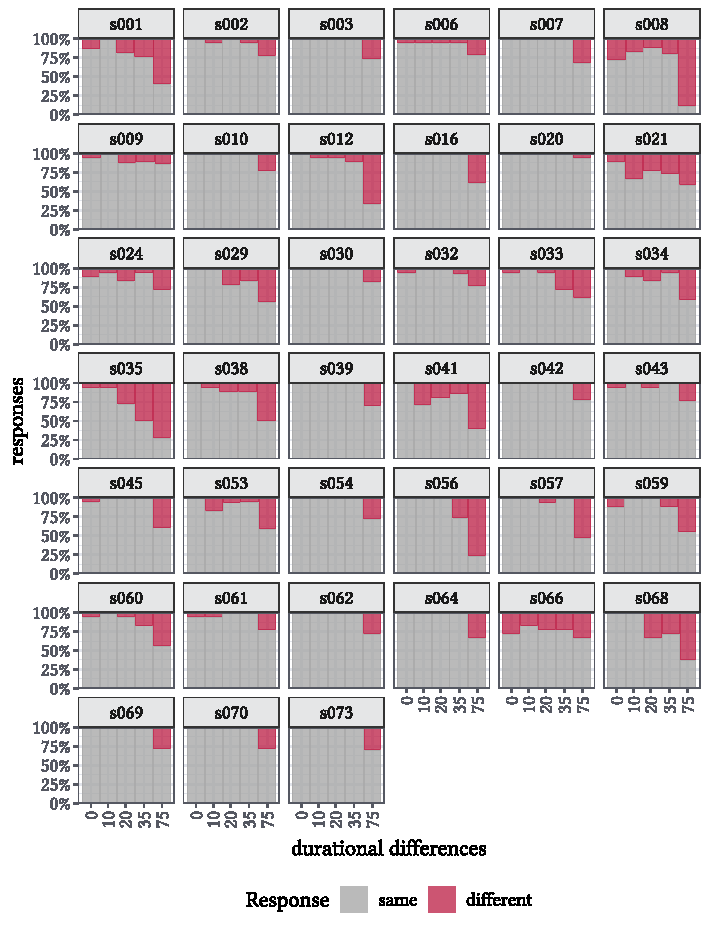
\includegraphics[]{figures/fig6.3.pdf}
    \caption{Error rates per subject for the same-different task for all durational differences. For a durational difference of 0 ms the error rate is represented by the part of the bar corresponding to \texttt{different}, while for all other durational differences the error rate is the given part of the pertinent bars corresponding to \texttt{same}.}
    \label{fig:6_3}
\end{figure}

One possible way to proceed from these descriptive findings is to fit a statistical model to the data. However, as has become visible, there are clear differences between subjects, which points towards another issue: Individuals may have different levels of conservativity. That is, a more conservative participant will less often respond with ``different", while a less conservative participant will more often respond with ``different", irrespective of the stimuli they hear. This intra-subject bias is neglected if one was to use the raw data, as was done in this section thus far.

A common way to factor in this participant bias is to make use of Signal Detection Theory (e.g. \cite{Macmillan1993,Macmillan2005}) and its measures. Signal Detection Theory can be applied in the analysis of any experiment in which two possible stimulus types are to be discriminated, i.e. in which error rates are the dependent variable of interest. The different measures of Signal Detection Theory have been used to analyse, among other things, recognition memory, lie detection, personnel selection, jury decision-making, medical diagnosis, industrial inspection, information retrieval, and congenital amusia (e.g. \cite{Stanislaw1999, Pfeifer2018}). Signal Detection Theory makes use of ``all four cells" of discriminative results as illustrated in the toy example in Table \ref{tab:6.9}.

\begin{table}\fontsize{10}{11}
\caption{Types of results for a discriminative task as described by type of stimulus and type of response. Values illustrate a toy example.}
\label{tab:6.9}
\centering
\begin{tabular}{lcccc}
\lsptoprule
\textbf{~}          & \multicolumn{2}{c}{response: different} & \multicolumn{2}{c}{response: same}  \\
\midrule
stimulus: different & \textsc{hit}         & 20                        & \textsc{miss}              & 5               \\
stimulus: same      & \textsc{false alarm} & 10                        & \textsc{correct rejection} & 15              \\
\lspbottomrule
\end{tabular}
\end{table}

To calculate the most commonly used Signal Detection Theory measure, a bias-free measure of subject sensitivity called $d'$, one must first calculate the hit rate $H$

\begin{equation}
\label{eq:H}
    H=\frac{HIT}{HIT+MISS}
\end{equation}

and the false alarm rate $F$

\begin{equation}
\label{eq:F}
    F=\frac{FALSE\ ALARM}{FALSE\ ALARM + CORRECT\ REJECTION}\ .
\end{equation}

Then, $d'$ can be computed as

\begin{equation}
\label{eq:dprime}
    d'=z(H)-z(F)
\end{equation}

\noindent where $z(.)$ is the Z-transform of either variable. However, $d'$ can only be meaningfully used if two assumptions regarding the decision variable are met (\cite{Stanislaw1999}). First, the signal and noise distributions are both normal. Second, the signal and noise distributions have the same standard deviation. In the present case, noise is equivalent to trials with two identical stimuli. If one of the assumptions is violated, $d'$ will vary with the response bias (\cite{Stanislaw1999}). Thus, it was decided to use an alternative measure, $A'$, instead. $A'$ is a nonparametric variant of $d'$ (\cite{Pollack1964}) and its values range between $0$ and $1$, where higher values indicate higher sensitivity, and $1$ indicates perfect performance. $H$ and $F$, as introduced above, are also used to calculate $A'$:

\begin{equation}
\label{eq:aprime}
    A'=0.5+\left [ sign(H-F)\frac{(H-F)^2+|H-F|}{4max(H,F)-4HF)}\right ],
\end{equation}

\noindent where the term $sign(H-F)$ is $+1$ if $H-F>0$, $0$ if $H=F$, and $-1$ otherwise. $max⁡(H,F$) equals either $H$ or $F$, whichever is greater (\cite{Stanislaw1999}). For the above toy example given in Table \ref{tab:6.9}, $A'$ then is

\begin{equation}
\label{eq:aprimeex}
    A'=0.5+\left [ \frac{(0.8-0.4)^2+|0.8-0.4|}{4*0.8-4*0.8*0.4)}\right ],
\end{equation}

\noindent that is, $A'$ has a value of about $0.79$. Thus, in the example, sensitivity is quite high.

In the following sections, I will first introduce the covariates used in the analysis of the same-different task data. Then, I will present the analysis of the data, including the calculation of $A'$ values from the raw data, and the statistical modelling of $A'$ as dependent variable.

\subsection{Covariates}\label{section06_2_1}

The set of covariates used in the analysis of the subject sensitivity data calculated from the same-different task results is more restricted than other sets of covariates in this book. As $A'$ values are calculated across all trials of a subject, item specific variables such as \textsc{typeOfS} (\texttt{non-morphemic} versus \texttt{plural}) and \textsc{typeOfWord} (\texttt{real word} versus \texttt{pseudoword}) cannot be used as covariates. However, analysing the raw data with chi-square tests strongly suggests that no significant difference for these variables were found ($p>0.05$ for all comparisons; see the supplementary material given in Chapter \ref{Supplementary Material}). As sensitivity may very well vary between subjects, an additional covariate on how regularly subjects play musical instruments was introduced. In the following, covariates used in previous studies of this book are described first. For these, definitions are briefly repeated for convenience and adapted to perception where necessary. Then, the newly introduced covariate is given. Finally, the covariate used as random effect is listed.

\textsc{age}. Subjects’ \textsc{age} was included as it may show an influence on hearing capabilities, with older subjects often experiencing a loss of hearing (e.g. \cite{Lee2013}).

\textsc{monoMultilingual}. To account for potential influences of other L1s besides English, the binary covariate \textsc{monoMultilingual} was introduced. 

\textsc{musicalInstrument}. It has been shown that advanced players of musical instruments show an increased performance of phonological perception and of detecting durational differences in speech (e.g. \cite{Anvari2002,Milovanov2009}). Thus, information on how regularly each subject plays a musical instrument was collected.

\textsc{subject}. \textsc{subject} ID was included to account for inter-speaker differences in perception.

Closer inspection of the newly introduced covariate, \textsc{musicalInstrument}, revealed that there was an uneven distribution of subjects across levels. That is, only 5\% (n = 8) of trials had \textsc{very often} as value for \textsc{musicalInstrument}, while 41\% (n = 64) had \textsc{never} as value. This skewed distribution is maintained by the levels in between, with 8\% \textsc{often} (n = 12), 20\% \textsc{sometimes} (n = 32), and 26\% \textsc{rarely} (n = 40). Due to the skewed distribution and the therefore small amount of data points for some levels, it was decided to drop \textsc{musicalInstrument} as a covariate. If there was an effect of \textsc{musicalInstrument} nonetheless, this should then be indirectly considered as part of the \textsc{subject} random effect.

\subsection{Overview of the data}\label{section06_2_2}

An overview of all variables used in the analysis of subject sensitivity and their distribution is given in Table \ref{tab:6.10}.

\begin{table}\fontsize{10}{11}
\caption{Summary of the dependent variable and the numerical and categorical predictors in the final data set.}
\label{tab:6.10}
\centering
\begin{tabular}{lllll} 
\lsptoprule
Dependent variable     & \multicolumn{1}{r}{Mean}        & \multicolumn{1}{r}{St. Dev.}                 & \multicolumn{1}{r}{Min}         & \multicolumn{1}{r}{Max}                       \\ 
\midrule
\textsc{aprime}                 & \multicolumn{1}{r}{0.323}       & \multicolumn{1}{r}{0.131}                    & \multicolumn{1}{r}{0.226}       & \multicolumn{1}{r}{0.904}                     \\ 
\midrule
Numerical predictors   & \multicolumn{1}{r}{Mean}        & \multicolumn{1}{r}{St. Dev.}                 & \multicolumn{1}{r}{Min}         & \multicolumn{1}{r}{Max}                       \\ 
\midrule
\textsc{age}                    & \multicolumn{1}{r}{23.000}      & \multicolumn{1}{r}{5.235}                    & \multicolumn{1}{r}{18.000}      & \multicolumn{1}{r}{39.000}                    \\ 
\midrule
Categorical predictors & Levels      & ~                        & ~           & ~                         \\ 
\midrule
\textsc{monoMultilingual}       & \multicolumn{2}{l}{\texttt{monolingual}:
  128} & \multicolumn{2}{l}{\texttt{multilingual}:
  28}  \\
\textsc{subject}                & 39          & ~                        & ~           & ~                         \\ 
\midrule
Explanatory variable   & Levels      & ~                        & ~           & ~                         \\ 
\midrule
\textsc{durDif}                 & \texttt{10 ms}:
  39 & \texttt{20 ms}:
  39              & \texttt{35 ms}:
  39 & \texttt{75 ms}:
  39               \\
\lspbottomrule
\end{tabular}
\end{table}

\subsection{Modelling subject sensitivity}\label{section06_2_3}

Using the formula for calculating $A'$ as given in Equation 14 and as implemented by the \texttt{psycho} package for R (\cite{Makowski2018}), $A'$ values for all subjects were computed. That is, for each subject, the results for the four durational differences 10 ms, 20 ms, 35 ms, and 75 ms were used to calculate an $A'$ value. This resulted in four $A'$ values per participant. The four durational differences are the predictor of interest in the regression modelling: \textsc{durDif}.

These $A'$ values then entered a regression analysis as dependent variable. As $A'$ assumes values in the standard unit interval $(0,1)$, regression models such as LMERs or gaussian GAMMs are not sufficient, because such models do not take into account the interval constraint of the dependent variable. As a workaround, one could transform the $A'$ values using, for example, a logit-transformation. However, this comes with several drawbacks (cf. \cite{Cribari2010}). It was thus decided to use beta regression as briefly introduced in Section \ref{section03_2_2} as the statistical tool of choice instead. Beta regression models assume that the dependent variable follows a beta distribution, i.e. that it assumes values in the open interval of $(0,1)$. Commonly, beta regression in R is done using the \texttt{betareg} package (\cite{Cribari2010}). However, the \texttt{betareg} implementation does not allow for random effects in its model specification. As it was plausible to assume inter-subject differences in the given context, the \texttt{mgcv} package (\cite{Wood2017}) and its GAMM implementation were made use of instead. While the default for GAMMs is to assume a dependent variable of gaussian distribution, GAMMs can also be specified for dependent variables following a beta distribution. This is what I call BGAMMs (see Section \ref{section03_2_2}).

A BGAMM was fitted with $A'$ as dependent variable. The predictor of interest, \textsc{durDif}, and the covariate \textsc{monoMulitlingual} were included as parametric effects. \textsc{age} was included as smooth term and \textsc{subject} was specified as random smooth term. Following the procedure introduced in Section \ref{section03_2_2}, the model was checked for issues of concurvity and of too few basis functions; no issues were found. The final data set as well as the analysis and results discussed in the following sections can be found in the supplementary material given in Chapter \ref{Supplementary Material}.

\section{Results}\label{section06_3}

An effect of \textsc{durDif} was found. Neither the effect of \textsc{monoMulitlingual} nor the effect of \textsc{age} reached significance. As anticipated, the random smooth of \textsc{subjct} reached significance. This was to be expected due to the vast differences between subjects already found in the raw data. The results of the BGAMM fitted to the $A'$ values are given in Table \ref{tab:6.11}. For the parametric terms, I provide the β estimates and the corresponding standard errors (SE), \textit{z}-values, and \textit{p}-values. For the smooth terms, the estimated degrees of freedom, the reference degrees of freedom, the χ\textsuperscript{2} values, and the \textit{p}-values are given.

\begin{table}\fontsize{10}{11}
\caption{Summary of the BGAMM fitted to the $A'$ values with \textsc{durDif} and \textsc{monoMultilingual} as parametric predictors, \textsc{age} as smooth term, and \textsc{subject} as random smooth term.}
\label{tab:6.11}
\centering
\begin{tabular}{lrrrr} 
\lsptoprule
Parametric Terms    & Estimate & SE     & z value & Pr(\textbar{}z\textbar{})  \\ 
\midrule
(Intercept)         & -1.008   & 0.079  & -12.818 & 0.000                      \\
\textsc{durDif20}            & 0.125    & 0.079  & 1.578   & 0.114                      \\
\textsc{durDif35}            & 0.206    & 0.077  & 2.676   & 0.007                      \\
\textsc{durDif75}            & 0.993    & 0.069  & 14.358  & 0.000                      \\
\textsc{monoMultilingual}    & -0.089   & 0.137  & -0.648  & 0.517                      \\ 
\midrule
Smooth Terms        & edf      & Ref.df & Chi.sq  & \textit{p}-value           \\ 
\midrule
\textsc{age}                 & 1.000    & 1.000  & 0.001   & 0.982                      \\ 
\midrule
Random Smooth Terms & edf      & Ref.df & Chi.sq  & \textit{p}-value           \\ 
\midrule
\textsc{subject}             & 28.400   & 36.000 & 144.904 & 0.000                      \\
\lspbottomrule
\end{tabular}
\end{table}

Figure \ref{fig:6_4} shows the partial effect of \textsc{durDif}. Participants show overall little sensitivity towards durational differences of 10 ms and 20 ms. For 35 ms a rather small but nonetheless significant increase in sensitivity is found as compared to the 10 ms difference. A clear increase in sensitivity is found for the durational difference of 75 ms as compared to the other differences. Thus, perceptibility of the 10 ms and 20 ms differences is rather low; the perceptibility of the 35 ms is significantly higher; and the perceptibility of the 75 ms difference is highest.

\begin{figure}
    \centering
    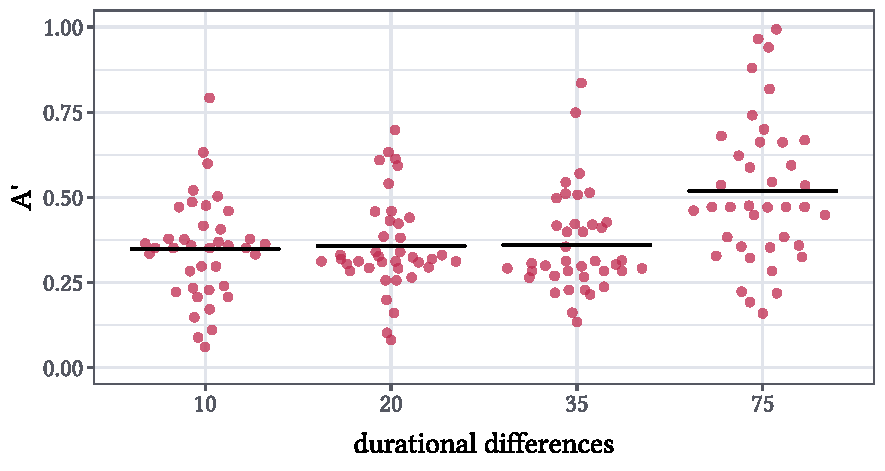
\includegraphics[]{figures/fig6.4.pdf}
    \caption{Partial effect of \textsc{durDif} as found by the BGAMM. The horizontal lines indicate the estimated $A'$ mean for each durational difference; the points illustrate subject-specific estimates.}
    \label{fig:6_4}
\end{figure}

The overall significant differences in sensitivity are given in Table \ref{tab:6.12}. Participants are significantly more sensitive towards the 75 ms difference as compared to all other durational differences. 

\begin{table}\fontsize{10}{11}
\caption{Significant contrasts found for the different /s/ durations contrasted in the same-different task. Significance codes: `***' $p < 0.001$, `**' $p < 0.01$, `*' $p < 0.05$.}
\label{tab:6.12}
\centering
\begin{tabular}{lrrrr} 
\lsptoprule
\textbf{~} & 10~ms & 20~ms & 35~ms & 75~ms  \\ 
\midrule
10~ms      & n.a.  & ~     & **    & ***    \\
20~ms      & ~     & n.a.  & ~     & ***    \\
35~ms      & ~     & ~     & n.a.  & ***    \\
75~ms      & ~     & ~     & ~     & n.a.   \\
\lspbottomrule
\end{tabular}
\end{table}

As shown by the subject-specific $A'$ estimates indicated by points in Figure \ref{fig:6_4}, however, inter-subject differences remain high. Especially the biggest durational difference, 75 ms, shows a discernible amount of variation. The raw by-subject $A'$ values as illustrated in Figure \ref{fig:6_5} confirm the notion of high inter-subject variability. While some subjects show little increase in sensitivity between the 10 ms and 75 ms differences (e.g. subjects ``s020" and ``s030"), other subjects show a clear increase in sensitivity (e.g. subjects ``s035" and ``s056"). Overall, a higher $A'$ value and thus sensitivity can be found for the 75 ms difference for most subjects.

\begin{figure}
    \centering
    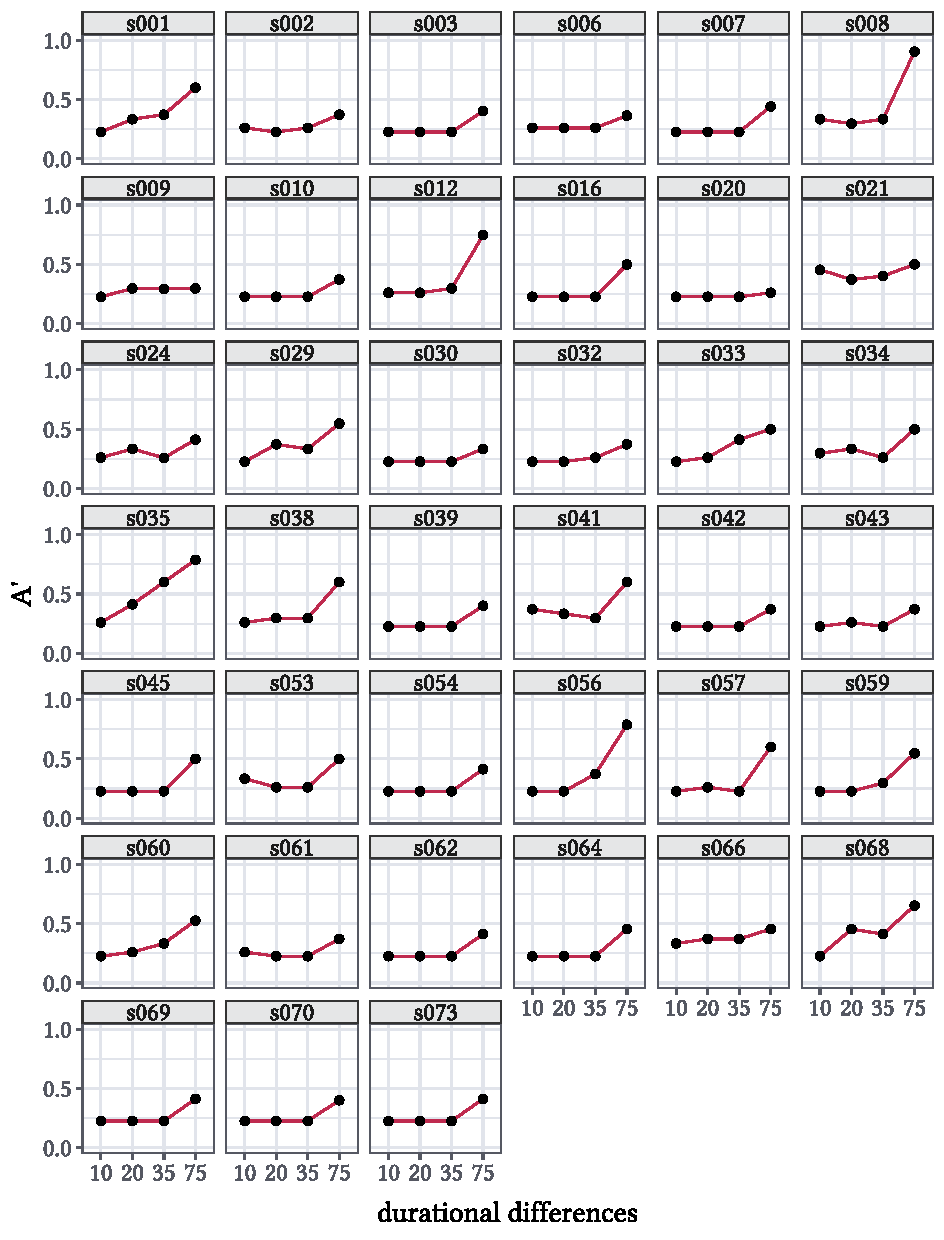
\includegraphics[]{figures/fig6.5.pdf}
    \caption{By-subject $A'$ values across all durational differences.}
    \label{fig:6_5}
\end{figure}

\section{Discussion}\label{section06_4}

Following previous studies on the perception of subphonemic differences, the present study investigated whether the durational differences between different types of word-final /s/ are perceptible. As such, this is the first study to look into the perception of phonologically identical but morphologically and phonetically different segments. Since real words as well as pseudowords were used as items, potential lexical effects were taken into account. It was found that durational differences in word-final /s/ as small as 10 ms and 20 ms are overall not well perceptible. Durational differences of 35 ms and 75 ms show significantly increased perceptibility, while a durational difference of 75 ms by far shows the greatest perceptibility.

What does this mean for the perceptibility of durational differences found for different types of word-final /s/? The durational differences found in \citet{Plag2017} and in the production study of Chapter \ref{chapter04} are given in Table \ref{tab:6.13}. None of the durational differences between the different types of /s/ is as high as 75 ms. However, considering the findings by \citet{Plag2017}, one would expect the differences between the non-morphemic /s/ and morphemic types of /s/ to be somewhat perceptible as these differences are all at least equal to or bigger than 35 ms. Taking into account the findings of Chapter \ref{chapter04}, only the durational difference between non-morphemic and clitic /s/ should be somewhat perceptible, as only this difference is close to or bigger than 35 ms. Considering both studies (\cite{Plag2017} and Chapter \ref{chapter04}), the findings indicate that at least some of the durational differences found between different types of /s/ are likely to be perceptible.

\begin{table}\fontsize{10}{11}
\caption{Durational differences between non-morphemic, plural, \mbox{is-,} and has-clitic /s/ in milliseconds found in \citet{Plag2017} and the production study presented in Chapter \ref{chapter04}.}
\label{tab:6.13}
\centering
\begin{tabular}{llcccc} 
\lsptoprule
\textbf{~}                           & ~           & non-morphemic & plural & \textit{is}-clitic & \textit{has}-clitic  \\ 
\midrule
\multirow{2}{*}{non-morphemic}       & Plag et al. & n.a.          & 35     & 57                 & 65                   \\
                                     & Chapter 4   & n.a.          & 14     & 31                 & 37                   \\ 
\midrule
\multirow{2}{*}{plural}              & Plag et al. & ~             & n.a.   & 22                 & 30                   \\
                                     & Chapter 4   & ~             & n.a.   & 17                 & 23                   \\ 
\midrule
\multirow{2}{*}{\textit{is}-clitic}  & Plag et al. & ~             & ~      & n.a.               & 8                    \\
                                     & Chapter 4   & ~             & ~      & n.a.               & 6                    \\ 
\midrule
\multirow{2}{*}{\textit{has}-clitic} & Plag et al. & ~             & ~      & ~                  & n.a.                 \\
                                     & Chapter 4   & ~             & ~      & ~                  & n.a.                 \\
\lspbottomrule
\end{tabular}
\end{table}

The significant increase in sensitivity of the 35 ms durational difference found in the present study is more or less in line with the findings by \citet{Klatt1975}. Recall that in their experiment, the just-noticeable difference to be perceived was 25 ms. That is, a durational difference between the 20 ms and 35 ms difference. The sensitivity between these two durational differences showed a significant increase, thus indicating that the just-noticeable difference to be perceived most likely lies within this range.

However, an overall increase in perceptibility was only found for the durational difference of 75 ms, for which the difference in sensitivity is significant for all comparisons. While I cannot give a definitive answer to the question of why this is the case, I want to propose two considerations. First, fricatives such as /s/ are not only perceived in terms of their duration but also by their centre of gravity, spectral peak location, spectral moments, noise duration, amplitude, and other acoustic features. In the present study, only one of many features – duration – was controlled for and manipulated. Perceptibility might be higher if all acoustic features are manipulated accordingly. Second, in their study, \citet{Klatt1975} found that durational differences in word-final position and in fricatives are less well perceptible as compared to other positions and consonants. As the present study investigated differences between fricatives in word-final position, perceptibility was expected to be rather low.

Let us now turn to the theoretical implications of the present results. How do the results relate to the two hypotheses that were tested? \textsc{H perc\textsubscript{1}}, the ``Abstractionist Hypothesis", assumes that listeners are not sensitive to subphonemic durational differences. As was illustrated, listeners show an increased sensitivity towards a durational difference of 35 ms and such a difference in duration was found between different types of word-final /s/ (e.g. \cite{Plag2017}; Chapter \ref{chapter04}). Also, none of the tested durational differences distinguishes between phonemes of English: No matter what its acoustic duration within a reasonable range, an /s/ is an /s/. Thus, the ``Abstractionist Hypothesis" is rejected.

As listeners were sensitive to subphonemic durational differences, \textsc{H perc\textsubscript{2}}, the ``Phonetic Detail Hypothesis", can potentially be confirmed. Assuming that fine-phonetic detail is perceived and stored, this hypothesis can most likely account for the present findings. Recent findings in neurobiology (\cite{Beach2021}) are especially compatible with the notion of hybrid models, as are part of this hypothesis. That is, brain response patterns in same-different tasks suggest that the perception process does not require loss of subphonemic detail. Instead, the neural representation of perceived speech includes phonemic and subphonemic detail. Yet, a final decision on whether theories underlying this hypothesis can account for the present findings can only be reached with pertinent implementations.

The results of the present study then give rise to a further question: Are durational differences between different types of word-final /s/ made use of in comprehension? This question will be investigated in Chapters \ref{chapter07} and \ref{chapter08}.
